\documentclass[../main/report.tex]{subfiles}
\begin{document}

\chapter{Results}

\section{Scalability of the Demolicious system}

The architecture of the Demolicious system easily scales to a larger number of proessors.
As there is a linear relationship between the number of streaming processors on chip and processor throughput, one can simply add more cores to increase performance.

Limiting factors to this scalability include:
\begin{enumerate}
  \item
    The more cores, the lower the clock frequency, as signal propagation time and fanout increases
  \item
    Space available on the chosen FPGA
  \item
    Power consumption constraints, as more cores increase active power consumption
\end{enumerate}

%LX45 usage
%
%8% lut, 1% slice
%
%12% lut, 2%slice fanout 4.57, 3.631 lut flipflop pairs
%
%
%28% LUT, 5% slice 8393 lut flip flop pairs
%
%
%6% Slice, 25% LUT, 36% occupied, 7958 lut flip flop pairs
%
%Not synthesizable

\todo{These numbers need regenerating. I'll do it tomorrow}
\begin{table}[H]
\begin{tabularx}{\textwidth}{cccccc}
\hline
Cores & Crit. path & Max freq. & Dynamic + quiescent power & LX16 & LX45 \\
\hline
\hline
2 / 2      & 17.103ns      & 58.469MHz & 0.272: 0.088 + 0.184 & \checkmark & \checkmark  \\
4 / 2     & 17.959ns      & 55.682MHz & 0.292: 0.107 + 0.184 & \checkmark & \checkmark \\
8 / 4   & 19.722ns      & 50.108MHz & 0.353: 0.168 + 0.186 &            & \checkmark \\
16 / 8     & X  & X & X          & \\
       &               &           &                   &    & \\
\hline
\end{tabularx}
\caption{Hardware configurations compared. Harvested from post place \& route static simulation.}
\label{table:scalability}
\end{table}

The 4-core design fits with room to spare on the LX16, but does not fit the 8-core design.
The LX45 shifts this up one notch, fitting the 8-core design, but being unable to place \& route the 16-core design.
For all processor designs, the critical path passes from the immediate field of the instruction through the ALU into the active register file.
This is something that could be increased drastically by pipelining the processor.

Figure \ref{table:scalability} shows that there is a negligible drop in maximum frequency from two to eight cores.
At 50.108MHz with 8 cores, the GPU has an instruction throughput of ~400 mips.
This compares favorably to the ~117 mips of the two-core architecture.

It does however come with a 100mAh increase in power draw.
Luckily this only constitutes a 30\% total increase in power, considerably less than the fourfold improvement in GPU throughput.
The decrease in execution time will allow both the host CPU and the GPU to enter lower power states quicker, reducing static power consumption.

\section{Screen frame rate}
Is it fast?

\section{Clock frequency}

\section{Video output}
The Demolicious system can output to a screen using HDMI.
The minimum resolution permitted by the HDMI protocol is $640\times480$,
but the size of the data memory limits the actual resolution to $512\times256$ pixels.
The rest of the screen is padded with a checker pattern.
Most of the time the output image is correct.
However, the output image is distorted under certain conditions.
\begin{figure}[H]
	\centering
	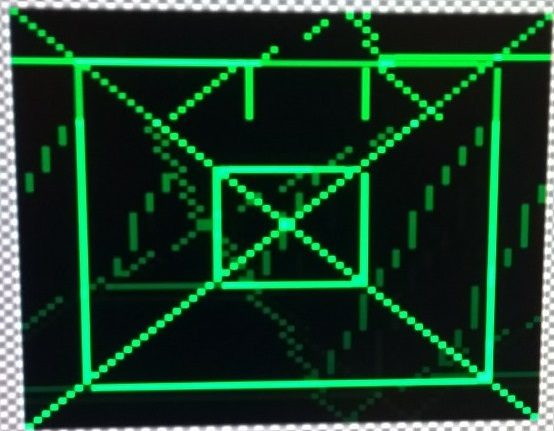
\includegraphics[width=0.3\textwidth]{diagrams/flicker.jpg}
	\caption{Flickering when running the tunnel kernel. This picture was exposed over two frames.}
	\label{fig:flickering}
\end{figure}
Some kernels exhibit intermittent flickering (Figure \ref{fig:flickering}).
The exact reason for why this occurs is unclear, but
it can be observed that the flicker contains parts of the last frame. 
This may be caused by a failure in the synchronization mechanism in the video unit.

Since the GPU has priority on memory access, the video unit may get starved for data.
When the video unit is starved the buffer containing pixels to output will underflow.
For the duration of the starve, a line containing the previous pixel on the bus will be displayed on the screen.



 
\end{document}
